\chapter{Constrained Optimisation on Graphs}

\section{Introduction}

There is an almost ubiquitous growing demand for mobile and wireless data, with consumers demanding faster speeds and better quality connections in more places. Consequently 4G is now being rolled out in the UK and US and with 5G being planned for 2020 and beyond \cite{Dahlman2014}.  

However, there is constrained amount of frequencies over which to transmit this information; and demand for frequencies that provide sufficient bandwidth, good range and in-building penetration is high.

Not all spectrum is used in all places and at all times, and judicious spectrum management, by developing approaches to use white spaces where they occur, would likely be beneficial.

Broadly, access to spectrum is managed in two, complementary ways, namely through licensed and licence exempt access. Licensing authorises a particular user (or users) to access a specific frequency band. Licence exemption allows any user to access a band provided they meet certain technical requirements intended to limit the impact of interference on other spectrum users.

A licence exempt approach might be particularly suitable for managing access to white spaces. Devices seeking to access white spaces need a robust mechanism for learning of the frequencies that can be used at a particular time and location. One approach is to refer to a database, which maps the location of white spaces based on knowledge of existing spectrum users. An alternative approach is for devices to detect white spaces by monitoring spectrum use. 

The advantages of spectrum monitoring \cite{akan2009cognitive} over maintaining a database of space-frequency data are the ability of networks to make use of low-cost low-power devices, only capable of making local (as opposed to national) communications, keeping the cost of the network low and  opportunistic channel usage for bursty traffic, reducing channel collisions in dense networks.

The realisation of any Cognitive Radio standard (such as IEEE 802.22 \cite{stevenson2009ieee}), requires the co-existence of primary (e.g. TV users) and secondary (everybody else who wants to use TVWS spectrum) users of the frequency spectrum to ensure proper interference mitigation and appropriate network behaviour. We note, that whereas TVWS bands are an initial step towards dynamic spectrum access, the principles and approaches we describe are applicable to other frequency bands - in particular it makes ultra-wideband spectrum sensing possible.

The challenges of this technology are that Cognitive Radios (CRs) must sense whether spectrum is available, and must be able to detect very weak primary user signals. Furthermore they must sense over a wide bandwidth (due to the amount of TVWS spectrum proposed), which challenges traditional Nyquist sampling techniques, because the sampling rates required are not technically feasible with current RF or Analogue-to-Digital conversion technology.

Due to the inherent sparsity of spectral utilisation, Compressive Sensing (CS) \cite{Candes2006} is an appropriate formalism within which to tackle this problem. CS has recently emerged as a new sampling paradigm allowing images to be taken from a single pixel camera for example. Applying this to wireless communication, we are able to reconstruct sparse signals at sampling rates below what would be required by Nyquist theory, for example the works \cite{mishali2010theory}, and \cite{tropp2010beyond} detail how this sampling can be achieved. 

However, even with CS, spectrum sensing from a single machine will be costly as the proposed TVWS band will be over a large frequency range (for instance in the UK the proposed TVWS band is from 470 MHz to 790 MHz, requiring traditional sampling rates of \textasciitilde 600 MHz). CS at a single sensor would still require high sampling rates. In this report we propose a distributed model, which allows a sensing budget at each node far below what is required by centralised CS.

The contributions of this report are that we propose a distributed model and solver pair which obviates the need for a Fusion Centre (centralised node) as in \cite{Zhang2011b}) to do any data processing. That is the solution is found in a distributed manner, by local computations and communications in with one-hop neighbours. This can be applied to other models which previously required central processing.

Moreover, our algorithm is simple to understand (it is an extension of the multi-block ADMM \cite{mota2013d}) and can be applied to other composite optimisation problems.

We also give new proofs of ideas found in \cite{mota2013d}. 

The structure of the report is as follows: in section \ref{sec:sensingmodel} we introduce the sensing model, in section \ref{sec:opt-on-graphs} we describe the distributed reconstruction algorithm \cite{mota2013d}, and finally in section \ref{sec:results} we show some results of the reconstruction quality of this model. 

\section{ADMM}

Given a set of measurements of the form

\begin{equation}
y = Ax + n 
\end{equation}

where \(x \in \re^n\) is an \(s\)-sparse vector we wish to recover, \(y \in \re^m\) is a set of noisy measurements, \(A \in \re^{m \times n}\) is a design or measurement matrix s.t. \(x\) is not in the null-space of \(A\), and \(z \in \re^m\) is AGWN. The signal \(x\) can be recovered by algorithms minimising the objective function:

\begin{equation}
L = \frac{1}{2} \vectornorm{Ax-y}_2^2 + \lambda\vectornorm{x}_1
\label{LASSO}
\end{equation}

where \(\lambda\) is a parameter which trades off the reconstruction accuracy and sparsity of \(x\): larger \(\lambda\) means sparser \(x\). 

One such algorithm is the alternating direction method of multipliers \cite{Boyd2010a}, (ADMM). This algorithm solves problems of the form

\begin{align}
\argmin_{x} f\left( x \right) + g\left(z\right) \nonumber
\\
\text{s.t } Ux +Vz = c
\label{admm}
\end{align}

where \(f\) and \(g\) are assumed to be convex function with range in \(\re\), \(U \in \re^{p \times n}\) and \(V\in \re^{p \times m}\) are matrices (not assumed to have full rank), and \(c \in \re^p\).

ADMM consists of iteratively minimising the augmented Lagrangian 

\begin{align*}
L_p\left(x, z, \eta\right) = f\left( x\right) +& g\left(z\right)+\eta^T\left(Ux+Vz-c\right) + \frac{\rho}{2}\|Ux+Vz-c\|_2^2
\label{admm_form}
\end{align*}

(\(\eta\) is a Lagrange multiplier), and \(\rho\) is a parameter we can choose to make \(g(z)\) smooth \cite{nesterov2005smooth}, with the following iterations:

\begin{align}
x^{k+1} &:= \argmin_{x} L_\rho\left(x,z^k,\eta^k\right)\\
z^{k+1} &:= \argmin_{z} L_\rho\left(x^{k+1},z,\eta^k\right)\\
\eta^{k+1} &:= \eta^{k} + \rho \left(Ux^{k+1} + Vz^{k+1} - c\right)
\label{admm_algo}
\end{align}

The alternating minimisation works because of the decomposability of the objective function: the \(x\) minimisation step is independent of the \(z\) minimisation step and vice versa.  

We illustrate an example, relevant to the type of problems encountered in signal processing.

ADMM can be formulated as an iterative MAP estimation procedure for the problem \eqref{LASSO}. We can write \eqref{LASSO} in constrained form as:

\begin{eqnarray}
\frac{1}{2}\|Ax-b\|_2^2 + \lambda\|z\|_1 \\
\text{s.t } z = x
\end{eqnarray}

i.e this is of the form \eqref{admm} with \( f\left(x\right) =\|Ax-y\|_2^2\), \(g\left(z\right) = \lambda\|z\|_1\), \(U=I\), \(V=-I\), and \(c=0\).

The associated (augmented) Lagrangian is:

\begin{equation}
L_\rho = \frac{1}{2}\|Ax-b\|_2^2 + \lambda\|z\|_1 + \eta\left(x-z\right) + \frac{\rho}{2}\|x-z\|^2
\label{eq:lasso-lagrangian}
\end{equation}

The ADMM iterations for LASSO, which can be found by alternately differentiating \eqref{eq:lasso-lagrangian} with respect to \(x\),\(z\) and \(\eta\), are (in closed form):

\begin{align}
x^{k+1} &:= \left(A^TA + \rho I\right)^{-1}\left(A^Ty +\rho\left( z^k - \eta^k/\rho\right)\right)\\
z^{k+1} &:= S_{\lambda/\rho}\left(x^{k+1} + \eta^k/\rho\right)
 \\
\eta^{k+1} &:= \eta^{k} + \rho\left(x^{k+1}-z^{k+1}\right)
\label{admm_algo_lasso}
\end{align}

where \(S_{\lambda/\rho}\left(\circ\right)\) is the soft thresholding operator: \(S_\gamma\left(x\right)_i = \mathrm{sign}(x_i)\left(|x_i| - \gamma\right)^+\).

These can be found differentiating \eqref{eq:lasso-lagrangian} with respect to \(x\) and \(z\) as follows:

\begin{align*}
\frac{\partial L}{\partial x } = -A^T\left(y-Ax\right) + \rho (x-z) + \eta
\end{align*}

as 

\begin{equation}
\frac{\partial}{\partial x} \vectornorm{F(x)}_2^2 = 2\left(\frac{\partial}{\partial x} F(x)\right) F(x) 
\label{dellx}
\end{equation}

by the chain rule, and \(\partial/\partial x (Ax) = -A^T\) (see the Matrix Cookbook) as differentiation exchanges a linear operator with its adjoint.

Setting \eqref{dellx} to zero and collecting like terms:

\begin{equation}
\left(A^TA + \rho I\right)x = A^Ty + \rho z - \eta
\end{equation}

so we find the optimal \(x\) is:

\begin{equation}
x = \left(A^T A + \rho I\right)^{-1}\left(A^Ty + \rho \left( z - \eta/\rho\right)\right)
\label{optx}
\end{equation}

note that this estimator is a weighted average of the ordinary least squares estimate (\(A^Ty\)) and a Gaussian prior. This is to be expected, as the minimisation problem w.r.t x is an \(l_2\)-regularised MAP problem.

for \(z > 0\)

\begin{equation}
\frac{\partial L} {\partial z} = \lambda + \rho (x-z) - \eta
\label{dellz-positive}
\end{equation}

from which we obtain:

\begin{equation*}
z = x + \frac{1}{\rho} ( \eta - \lambda )
\end{equation*}

since \(z>0\) then \(x + \frac{1}{\rho} ( \eta - \lambda I) > 0\) when \(x + \frac{\eta}{\rho} > \frac{\lambda}{\rho}\).

Similarly for \(z < 0\):

\begin{equation}
\frac{\partial L} {\partial z} = -\lambda + \rho (x-z) 
\label{dellz-negative}
\end{equation}

setting \eqref{dellz-negative} to zero we obtain:

\begin{equation*}
z = x + \frac{1}{\rho}(\eta + \lambda)
\end{equation*}

since \(z<0\) then \(x + \frac{1}{\rho} ( \eta + \lambda ) < 0\) when \(x + \frac{\eta}{\rho} < - \frac{\lambda}{\rho}\).

at \(z=0\) we find:

\begin{equation*}
-\frac{\lambda}{\rho} \leq x + \frac{\eta}{\rho} \leq \frac{\lambda}{\rho}
\end{equation*}

i.e.

\begin{equation}
\mid x+ \frac{\eta}{\rho}\mid \leq \frac{\lambda}{\rho}
\label{zbounds}
\end{equation}

combining \eqref{dellz-negative}, \eqref{dellz-positive}, \eqref{zbounds} together we find the optimal \(z\) is:

\begin{equation}
z = \mathrm{sign}(x+\frac{\eta}{\rho})\text{ }\mathrm{max}\left( \mid x+\frac{\eta}{\rho} \mid - \frac{\lambda}{\rho} ,0\right)
\label{optz}
\end{equation}

Together \eqref{optx}, \eqref{optz} and the third step of \eqref{admm_algo_lasso} constitute the steps of the ADMM algorithm.

This algorithm has a nice statistical interpretation: it iteratively performs ridge regression, followed by shrinkage towards zero. This is the MAP estimate for \(x\) under a Laplace prior.

The soft-thresholding operator can be derived by considering the MAP estimate of the following model:

\begin{equation}
y = x + w
\end{equation}

where \(x\) is some (sparse) signal, and \(w\) is additive white Gaussian noise. We seek

\begin{equation}
\hat{x} = \arg\max_x \pr_{x|y}{\left(x|y\right)}
\end{equation}

This can be recast in the following form by using Bayes rule, noting that the denominator is independent of \(x\) and taking logarithms:

\begin{equation}
\hat{x} = \arg\max_x \left[\log{\pr_{w}{\left(y-x\right)}}+\log{\pr{\left(x\right)}}\right]
\label{hatx}
\end{equation}

The term \(\pr_{n}{\left(y-x\right)}\) arises because we are considering \(x+w\) with \(w\) zero mean Gaussian, with variance \(\sigma_n^2\). So, the conditional distribution of \(y\) (given \(x\)) will be a Gaussian centred at \(x\).

We will take \(\pr{\left(x\right)}\) to be a Laplacian distribution:

\begin{equation}
\pr{\left(x\right)} = \frac{1}{\sqrt{2}\sigma}\exp{-\frac{\sqrt{2}}{\sigma}|x|}
\end{equation}

Note that \( f\left(x\right) = \log{\pr_x{ \left( x \right)}} ~ -\frac{\sqrt{2}}{\sigma} |x| \), and so by differentiating \( f'\left(x\right) = -\frac{\sqrt{2}}{\sigma} \mathrm{sign}\left(x\right) \)

Taking the maximum of \ref{hatx} we obtain:

\begin{equation}
\frac{y-\hat{x}}{\sigma^2_n}-\frac{\sqrt{2}}{\sigma}sign(x) = 0
\end{equation}

Which leads the soft thresholding operation defined earlier, with \(\gamma = \frac{\sqrt{2}\sigma^2_n}{\sigma}\) as (via rearrangement):

$$
y =  \hat{x} + \frac{\sqrt{2}\sigma^2_n}{\sigma}\mathrm{sign}\left(x\right)
$$

or

$$
\hat{x}\left(y\right) = \mathrm{sign}(y)\left(y - \frac{\sqrt{2}\sigma^2_n}{\sigma}\right)_+
$$

i.e \(S_\gamma(y)\).

\subsection{The Proximity Operator}
The Proximity Operator for a closed, convex, and proper function \(f\) (the set of all such functions will be denoted \(\Gamma\) in a Hilbert space \(\mathcal{H}\) is defined as:

\begin{definition}[Proximity Operator]
\begin{equation}
\mathrm{Prox}_f\left(y\right) :=  \argmin_{y \in \mathcal{H} } f\left(y\right) + \frac{1}{2}\vectornorm{y-x}^2
\end{equation}
\end{definition}

Intuitively the Proximity Operator approximates a point \(x\) by another point \(y\), that is close in the mean-square sense under the penalty \(f\).

The \(\mathrm{Prox}\left(\circ\right)\) operator exists for closed and convex \(f\) as \(\left(y\right) + \frac{1}{2}\vectornorm{y-x}^2\) is closed with compact level sets and is unique as \(\left(y\right) + \frac{1}{2}\vectornorm{y-x}^2\) is strictly convex.

The corresponding Moreau envelope is defined as 

\begin{definition}[Moreau Envelope]
\begin{equation}
\mathrm{M}_f\left(y\right) :=  \min_{y \in \mathcal{H}} f\left(y\right) + \frac{1}{2}\vectornorm{y-x}^2
\end{equation}
\end{definition}

The Moreau envelope is a strict generalisation of the squared distance function. \(\mathrm{M}_f\) is real valued - even when \(f\) takes the value \(\infty\), whilst \(\mathrm{Prox}_f \) is \(\mathcal{H}\)-valued. 

\subsubsection{Properties}
\begin{theorem}[Moreau '65]
Let \(f \in \Gamma\) and \(f^*\) be its Fenchel conjugate. Then the following are equivalent:
\begin{itemize}
\item \(z = x+y, y \in \partial f\left(x\right)\)
\item \(x = \mathrm{Prox}_f\left(z\right), y = \mathrm{Prox}_{f^*}\left(z\right)  \)
\end{itemize}
\end{theorem}

\begin{theorem}[Moreau '65]
Let \(f \in \Gamma\). Then for all \(z \in \mathcal{H}\)
\begin{itemize}
\item \( \mathrm{Prox}_f\left(z\right) + \mathrm{Prox}_{f^*}\left(z\right) = z   \)
\item \( \mathrm{M}_f\left(z\right)  + \mathrm{M}_{f^*}\left(z\right)  = \frac{1}{2}\vectornorm{z}^2 \)
\end{itemize}
\end{theorem}

\begin{theorem}[Moreau '65]
The Moreau envelope is (Frechet) differentiable, with 
\begin{equation}
\nabla \mathrm{M}_f = Id - \mathrm{Prox}_{f} = \mathrm{Prox}_{f^*}
\end{equation}
\end{theorem}

\begin{theorem}[Moreau '65]
\( \mathrm{Prox}_f : \left(\mathcal{H}, \vectornorm{\circ}\right) \leftarrow \left(\mathcal{H}, \vectornorm{\circ}\right) \) is 1-Lipchitz continuous.
\end{theorem}

\subsubsection{Motivation}
We are solving problems of the following form:

\begin{align}
&\min_{x \in \mathcal{H}} f\left(x\right) + g\left(z\right)\\
&\text{s.t } x - z = 0
\end{align}

with \(f, g \in \Gamma\). To solve this problem we form the augmented Lagrangian: 

\begin{align*}
L_p\left(x, z, \eta\right) = f\left( x\right) +& g\left(z\right)+\eta^T\left(Ux+Vz-c\right) + \frac{\rho}{2}\|Ux+Vz-c\|_2^2
\end{align*}

and then performing the following iterative minimisation:

\begin{align}
x^{k+1} &:= \argmin_{x} L_\rho\left(x,z^k,\eta^k\right)\\
z^{k+1} &:= \argmin_{z} L_\rho\left(x^{k+1},z,\eta^k\right)\\
\eta^{k+1} &:= \eta^{k} + \rho \left(x^{k+1} + z^{k+1}\right)
\end{align}

i.e. 

\begin{align}
x^{k+1} &:= \argmin_{x} \left( f\left(x\right) + \eta^{kT}x + \frac{\rho}{2}\vectornorm{x - z^k}^2 \right) \\
z^{k+1} &:= \argmin_{z} \left( g\left(z\right) - \eta^{kT}z + \frac{\rho}{2}\vectornorm{x^{k+1} - z}^2 \right)\\
\eta^{k+1} &:= \eta^{k} + \rho \left(x^{k+1} + z^{k+1}\right)
\end{align}

pulling the linear terms into the quadratic ones we get:

\begin{align}
x^{k+1} &:= \argmin_{x} \left( f\left(x\right) +  \frac{\rho}{2}\vectornorm{x - z^k + \left(1/\rho\right)\eta^k}^2 \right) \\
z^{k+1} &:= \argmin_{z} \left( g\left(z\right) +  \frac{\rho}{2}\vectornorm{x^{k+1} - z - \left(1/\rho\right)\eta^k}^2 \right)\\
\eta^{k+1} &:= \eta^{k} + \rho \left(x^{k+1} + z^{k+1}\right)
\end{align}

i.e.

\begin{align}
x^{k+1} &:= \mathrm{Prox}_f \left( z^k - u^k\right)\\
z^{k+1} &:= \mathrm{Prox}_f \left(x^{k+1} + u^k\right)  \\
u^{k+1} &:= u^{k} + \left(x^{k+1} + z^{k+1}\right)
\end{align}

with \(u^k = \left(1/\rho\right) \eta^k\).

The motivation for the Proximal operator should now be clear: to perform the minimisation we simply calculate the proximal operator of each of the functions at each step. For many functions found in Statistics (e.g. the \(l_p\) norms, this can be found in closed form, and so ADMM presents a particularly attractive method for finding MAP solutions to regularised statistical problems.

\subsubsection{Examples}

\begin{example}[Indicator]
From the definition 

\begin{align}
\mathrm{Prox}_I\left(x\right) &:=  \argmin_y I_C(y) + \frac{1}{2}\vectornorm{y-x}^2 \\
& = \argmin_{y \in C} \frac{1}{2}\vectornorm{y-x}^2 \\
& = P_C\left(x\right)
\end{align}

where \(I_C(y)\) is the indicator of some set \(C\) and \(P_C\) is the projection operator onto that set.
\end{example} 

\begin{example}[\(l_2\) norm]
For \(f(y) = \frac{\mu}{2}\vectornorm{y}^2\) the \(\mathrm{Prox}\) operator is:

\begin{align}
\mathrm{Prox}_f\left(x\right) &:=  \argmin_y \frac{\mu}{2}\vectornorm{y}^2 + \frac{1}{2}\vectornorm{y-x}^2 \\
& = \frac{1}{1+\mu}x
\end{align}
\end{example}

\begin{example}[\(l_1\) norm]
\(f = \|x\|_1\)

\begin{equation}
\mathrm{Prox}_f\left(x\right) := \mathrm{sign}(x_i)\left(|x_i| - \gamma\right)^+ = S_\gamma\left(x\right)_i 
\end{equation}
\end{example}

\begin{example}[Elastic Net]
Consider

\begin{equation}
f(x) = \lambda\|x\|_1 + \mu \vectornorm{x} 
\end{equation}

\begin{equation}
\mathrm{Prox}_f\left(x\right) := \frac{\lambda}{1+\mu} S_\gamma\left(x\right)_i 
\end{equation}
\end{example}

\begin{example}[Fused Lasso]
Consider

\begin{equation}
f(x) = \|x\|_1 + \sum_{i=1}^{d-1} \left( x_i - x_{i-1} \right) 
\end{equation}

i.e the sum of the \(l_1\) and \(TV\) norms

\begin{equation}
\mathrm{Prox}_f\left(x\right) := \mathrm{Prox}_{l_1} \circ \mathrm{Prox}_{TV} =  S_\gamma\left(\mathrm{Prox}_{TV}\right)_i 
\end{equation}
\end{example}

\begin{example}[Consensus]

Suppose we want to solve a problem such as:

\begin{equation*}
\begin{aligned}
& \underset{x}{\text{minimize}}
& & \sum_i f_i\left( x \right) \\
\label{consensus}
\end{aligned}
\end{equation*}

this could arise in statistical computing where \(f_i\) would be the loss function for the \(i^th\) block of training data. We can write the problem for distributed optimisation as:

\begin{equation*}
\begin{aligned}
& \underset{x}{\text{minimize}}
& & \sum_i f_i\left( x_i \right) \\
& \text{subject to}
& & x_i - z = 0
\label{admm_consensus}
\end{aligned}
\end{equation*}

where \(x_i\) are local variables (for example local to each node in a spectrum sensing) and \(x_i - z = 0\) are the consensus constraints. Consensus and regularisation can be achieved by adding a regularisation term \(g\left(z\right)\) - for example \(g\left(z\right) = \lambda||x||_1\) corresponds to the LASSO, and the \(f_i\) would be \(f_i = ||A_ix_i - b||_2^2\). 

As per the previous sections, we form the Augmented Lagrangian:

\begin{equation}
L_\rho\left(x,y\right) = \sum_i^n \left(f_i\left( x_i \right) + y_i^T\left(x_i-z\right) + \frac{\rho}{2}\|x_i-z\|_2^2\right)
\end{equation}

The ADMM iterations for this Lagrangian are:

\begin{align}
x_i^{k+1} &:= \argmin{x_i} \left(f_i\left( x_i \right) + y_i^{kT}\left(x_i-z\right) + \frac{\rho}{2}\|x_i-z\|_2^2\right)\\
z^{k+1} &:= \frac{1}{n}\sum_i^n \left(x_i^{k+1} + \left(1\rho\right)y_i^k\right)\\
y_i^{k+1} &:= y_i^{k} + \rho \left(x_i^{k+1} - z^{k+1} \right)
\label{consensus_iterations}
\end{align}

The \(z^{k+1}\) iteration is analytic as we're minimising the squared norm of \(x_i - z\) - so we average. With \(\|x\|_1\) regularisation we perform soft-thresholding after the \(z\) update.

At each iteration the sum of the dual variables \(y_i\) is zero, so the algorithm can be simplified to:

\begin{align}
x_i^{k+1} &:= \argmin{x_i} \left(f_i\left( x_i \right) + y_i^{kT}\left(x_i-\bar{x}^k\right) + \frac{\rho}{2}\|x_i-\bar{x}^k\|_2^2\right)\\
y_i^{k+1} &:= y_i^{k} + \rho \left(x_i^{k+1} - z^{k+1} \right)
\label{simple_consensus_iterations}
\end{align}
 
where

\begin{equation}
\bar{x}^k = \frac{1}{n} \sum_i^n x_i^k
\end{equation}

This algorithm can be summarised as follows: in each iteration

\begin{itemize}
\item gather \(x^k\) and average to get \(\bar{x}^k\)
\item scatter the average to nodes
\item update \(y_i^k\) locally
\item update \(x_i\) locally
\end{itemize}

Each agent is minimising it's own function, plus a quadratic term (the squared norm) which penalises the agent from moving too far from the previous average.

Note that the 'gather' stage doesn't require a central processor - this can be done in a distributed manner also.
\end{example}

\subsection{Statistical Interpretation}
At each step \(k\) of the algorithm each agent is minimising it's own loss function, plus a quadratic.
This has a simple interpretation: we're doing MAP estimation under the prior \(\mathcal{N}\left(\bar{x}^{k} + \left(1\rho\right)y_i^k, \rho I\right)\). I.e. the prior mean is the previous iteration's consensus shifted by node \(i\) disagreeing with the previous consensus. 

\subsection{Acceleration}


\section{Constrained Optimisation on Graphs}\label{sec:opt-on-graphs}

We model the network of sensors as an undirected graph \(G = \left(V,E\right)\), where \(V = \{1 \ldots J\}\) is the set of vertices, and \(E = V \times V\) is the set of edges. An edge between nodes \(i\) and \(j\) implies that the two sensors can communicate. The set of nodes that node \(i\) can communicate with is written \(\mathcal{N}_i\) and the degree of node \(i\) is \(D_i = |\mathcal{N}_i|\). 

Individually nodes make the following measurements (as discussed in section \ref{sec:sensingmodel}):

\begin{equation}
\vec{y}_p = \vec{A}_p\vec{x} + \vec{n}_p
\end{equation}

where \(\vec{A}_p\) is the \(p^{th} \) row of the sensing matrix from \eqref{system}, and the system \eqref{system} is formed by concatenating the individual nodes' measurements together.

We assume that a proper colouring of the graph is available: that is, each node is assigned a number from a set \(C = \{1 \ldots c \} \), and no node shares a colour with any neighbour. This is so that nodes may communicate in colour order, as opposed to communicating individually thus reducing the total number of communication rounds required. 

To find the \(\vec{x}\) we are seeking (the solution to the linear system, \ref{system}), to each node we give a copy of \(\vec{x}, \vec{x}_p\) and we constrain the copies to be identical across all edges in the network. Each node, thus has a separate optimisation to solve, subject to the constraint that it is consistent with its neighbours.

The problem then is to solve:

\begin{align}
\argmin_{\bar{x}} \sum_{c=1}^C \sum_{j \in c} f\left(x_j\right) + \frac{\lambda}{J} g\left(x_j\right) \nonumber \\ 
\text{ and } x_i = x_j \text{ if } \{i,j\} \in E \nonumber \\
\text{ and } x_i = z_i \text{ } \forall i \in \{1, \ldots, C\}
\label{constrainedbp}
\end{align}

with a particular special case being:

\begin{align}
\argmin_{\bar{x}} \sum_{c=1}^C \sum_{j \in c} \|A_jx_j - y_j\|_2^2 + \frac{\lambda}{J}\|z\|_1 \nonumber \\ 
\text{ and } x_i = x_j \text{ if } \{i,j\} \in E \nonumber \\
\text{ and } x_i = z_i \text{ } \forall i \in \{1, \ldots, C\}
\label{constrainedbp}
\end{align}

i.e. \(f = \vectornorm{x}_2^2\) and \(g = \vectornorm{x}_1\).

That is, at each node we minimise a Lasso functional constrained to be consistent across edges but that is separable in the \(l_2\) and \(l_1\) norms.

We can write the global optimisation variable as \(\bar{x}\), which collects together \(C\) copies of a \(n\times 1\) vector \(\vec{x}\):

\begin{defn}
We define vectors \(x_c\), where \(c = 1,\ldots , C\) and write the vector of length \(nJ\):
\begin{equation}
\bar{x} = \sum_{c=1}^C w_c \otimes x_c = \left[x_{c(1)}^T, \ldots	, x_{c(J)}^T\right]^T
\label{barxc}
\end{equation}
where \(w_{c(i)} = \mathbb{I}(c(i) = c)\), \(\mathbb{I}\) is the indicator function, and we have written \(c(i)\) for the colour of the \(i\)th node.
\end{defn}

These constraints can be written more compactly by introducing the node-arc incidence matrix B: a \(V\) by \(E\) matrix where each column is associated with an edge \(\left(i,j\right) \in E\) and has \(1\) and \(-1\) in the \(ith\) and \(jth\) entry respectively. Figures \eqref{efig:ex-network} and \eqref{fig:incidence-matrix} show examples of a network and it's associated incidence matrix.

The constraint \(x_i = x_j \text{ if } \{i,j\} \in E \) can now be written 

\begin{equation}
\sum_{c=1}^C\left(B_c^T \otimes I_n\right)\bar{x}_c = 0
\label{compact-constraints}
\end{equation}

note that \(\left(B^T\otimes I_n \right) \in \re^{nE \times nJ}\). Together \eqref{barxc} and \eqref{compact-constraints}, suggests that the problem \eqref{constrainedbp} can be re-written as:

\begin{align}
\argmin_{\bar{x}} \sum_{c=1}^C \sum_{j \in C_c} f\left(x_j\right) + \frac{\lambda}{J} g\left(z_j\right)
\nonumber \\
\text{ s.t. } \sum_{c=1}^C\left(B_c^T \otimes I_n\right)\bar{x}_c = 0 \nonumber \\
\text{ and } \bar{x}_c - \bar{z}_c = 0
\label{constrainedbp1}
\end{align}

where \(\beta = \frac{\lambda}{J}\).

The global Augmented Lagrangian \cite{Boyd2010a}
 for the problem \eqref{constrainedbp1} can be written down as:

\begin{align}
L_\rho = \sum_{c=1}^C  ( \sum_{j \in c} & f\left(x_j\right) + \frac{\lambda}{J} g\left(z_j\right)  + \nonumber \\ & + \theta^T\left(\bar{x}_j - \bar{z}_j\right)  +  \frac{\rho}{2}\vectornorm{\bar{x}_j-\bar{z}_j}_2^2 ) + \nonumber \\  & + \eta^T\left(B_c^T \otimes I_n\right)\bar{x}_c + \frac{\rho}{2}\vectornorm{\sum_{c=1}^C\left(B_c^T \otimes I_n\right)\bar{x}_c}_2^2
\label{aug-lagrange}
\end{align}

This is, superficially, similar to the Augmented Lagrangian for the Lasso problem \cite{Boyd2010a}[Section 6.4]. That is, the terms indexed by \(j\) are a straightforward Lasso problem, constrained by edge-wise variables (indexed by \(c\)) forcing consistency across the network. However, the problem (as currently written) is not separable across the edges of the network as the final and penultimate term represent the constraint that the nodes agree on their estimates across edges. 

To make it possible that \ref{aug-lagrange} can be posed  as a constrained optimisation problem at each node, we introduce the following variable (so that the the final term of \ref{aug-lagrange} is separable across edges of the graph):

\begin{defn}
\begin{align*}
u &:= \left(B^T \otimes I_n\right)\bar{x} \\
& = \left(B^T \otimes I_n\right)\sum_{c=1}^C w_c \otimes x_c \\
& = \sum	_{c=1}^C B_c^T\otimes x_c
\end{align*}
where we have used the definition \eqref{barxc} in the second line, and the property of Kronecker products \((A\otimes C)(B \otimes D) = (AB \otimes CD)\) between the second and third lines, and we write \(B_c = w_c^TB\).
\end{defn}

\begin{figure}[h]
\centering
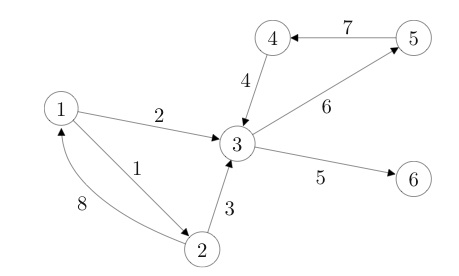
\includegraphics[height = 5 cm]{network-ex-incidence-mat.jpg}
\caption{An example of a network}
\label{efig:ex-network}
\end{figure}

\begin{figure}[h]
\centering
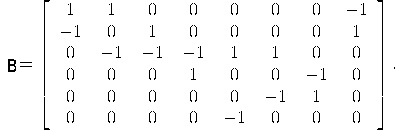
\includegraphics[height = 3 cm, width = 7cm]{ex-incidencematrix1.png}
\caption{The incidence matrix associated with Figure \eqref{efig:ex-network}}
\label{fig:incidence-matrix}
\end{figure}

The terms \(\|\sum_{c=1}^C\left(B_c^T \otimes I_n\right)\bar{x}_c\|^2\) and \( \eta^T\left(B_c^T \otimes I_n\right)\bar{x}_c \) of \eqref{aug-lagrange}, can be decomposed across edges, using the following lemma:

\begin{lemma}[Edge Decomposition]
\begin{equation}
\vectornorm{\sum_{c=1}^C\left(B_c^T \otimes I_n\right)\bar{x}_c}^2 = \sum_{j \in C_1}\left( D_j\vectornorm{x_j}_2^2 - \sum_{k \in N_j} x_j^Tx^k\right)
\end{equation}

and

\begin{equation}
\eta^T\sum_{c=1}^C\left(B_c^T \otimes I_n\right)\bar{x}_1 = \sum_{l\in C_c} \sum_{m\in N_l}sign\left(m-l\right)\eta_{ml}^T x_l
\end{equation}

where \(\eta\) is decomposed edge-wise: \(\eta = \left(\ldots, \eta_{ij},\ldots\right)\), such that \(\eta_{i,j} = \eta_{j,i}\), and is associated with the constraint \(x_i = x_j\).


\begin{proof}

\begin{align*}
u^Tu &= \sum	_{c_1=1}^C \sum	_{c_2=1}^C  \left(B_{c_1} \otimes x_{c_1}^T\right) \left(B_{c_2}^T \otimes x_c\right) \\
&= \sum_{c_1, c_2} B_{c_1}B_{c_2}^T \otimes x_{c_1}^Tx_{c_2}
\end{align*}

\(BB^T\) is a \(J \times J\) matrix, with the degree of the nodes on the main diagonal and \(-1\) in position \(\left(i,j\right)\) if nodes \(i\) and \(j\) are neighbours (i.e \(BB^T\) is the graph Laplacian). Hence, since we can write \(B_{c_1}B_{c_2}^T = w_{c_1}^TBB^Tw_{c_2}\), the trace of \(B_{c_1}B_{c_1}^T\) is simply the sum of the degrees of nodes with colour 1. 

For \(c_1 \neq c_2\),  \(B_{c_1}B_{c_2}^T\) corresponds to an off diagonal block of the graph Laplacian, and so counts how many neighbours each node with colour 1 has.

Finally, note that \(\eta \in \re^{nE}\) and can be written:

\begin{equation}
\eta = \sum_{c=1}^C w_c \otimes \eta_c
\end{equation}
where \(\eta_c\) is the vector of Lagrange multipliers associated across edges from colour \(c\). Now

\begin{align*}
\eta^Tu = \sum_{c_1=1}^C\sum_{c_2=1}^C w_{c_1}Bw_{c_2} \otimes \eta_{c_1}^Tx_c
\end{align*}
by the properties of Kronecker products, and the definition of \(B_c\). For \(c_1=c_2\), \(\eta^Tu\) is zero, as there are no edges between nodes of the same colour b definition. For \(c_1\neq c_2\), \(\eta^Tu\) counts the edges from \(c_1\) to \(c_2\), with the consideration that the edges from \(c_2\) to \(c_1\) are counted with opposite parity.
\end{proof}
\end{lemma}



Adding together this with the lemma, lets us write \eqref{aug-lagrange} as:

\begin{align}
L_\rho = \sum_{c=1}^C\sum_{j \in C_c} &\left( f\left(x_j\right) + \beta g\left(z_j\right)\right) + \nu^Tx_j \nonumber \\
& \text{        } \theta\left(x_j - z_j\right) + \frac{\rho}{2}D_i\vectornorm{x_j}^2 + \frac{\rho }{2}\|x_j-z_j\|^2
\label{generic-iterations}
\end{align}

where we have defined:

\begin{equation}
\nu_i = \left(\sum_{k \in \mathcal{N}_i} sign\left(k-i\right)\eta_{\{i,k\}} - \rho x_k \right)
\end{equation}

this is a rescaled version of the Lagrange multiplier, \(\eta\), which respects the graph structure. 

Then by differentiating \eqref{generic-iterations} with respect to \(x_j\) and \(z_j\) we  can find closed forms for the updates as:

\begin{thm}
\begin{align}
x_j^{k+1} &:= \left(A_j^TA_j + (\rho D_J + 1) I\right)^{-1}\left(A_j^Ty_j +  z^k - \nu^{kT}\right)\\
z_j^{k+1} &:= S_{\beta/\rho}\left(x_j^{k+1} \right)
 \\
\theta_j^{k+1} &:= \theta_j^{k} + \rho \left(x^{k+1}-z^{k+1}\right) \\
\eta_j^{k+1} &:= \eta_j^k + \rho\left(\sum_{m \in N_j} z_m^k - z_j^k\right)
\label{dadmm_algo_lasso}
\end{align}
\end{thm}

This algorithm can be thought of as follows: each node performs an iteration of (non multi-block) ADMM - i.e. each node solves an approximate Gaussian least-squares problem and then soft-thresholds - and then exchanges the result of this computation with its one-hop neighbours. This explains the inclusion of an extra Lagrange multiplier: the multiplier \(\theta\) controls how far each node moves from its previous estimate in each iteration, whilst the multiplier \(\eta\) enforces consistency between nodes. Note that there is no communication of data between the nodes - only the result the computation in each round.
